\section{Tests}

\subsection{Während der Entwicklung}
\label{chapter:implementation:tests}
Für das Testen während der Entwicklung wurde die Extension \emph{swagger-ui} verwendet. 
Erreichbar ist die Testresource unter \emph{http://localhost:8080/q/swagger-ui/}. 
In dem lilanem Rechteck lässt sich der Pfad erkennen, während sich in dem rotem Rechteck der Button zum ausprobieren befindet. 
Nachdem das "Try it out" geklickt wurde, können die benötigten Werte für den Endpoint eingegeben werden (siehe Abb. \ref{fig:implementation:swaggerui}). 
Der Pfad kann bei GET-Requests einfach in einem Browserfenster eingegeben werden und liefert dieselbe Antwort, wie das Tool. 

\begin{figure}
    \centering
    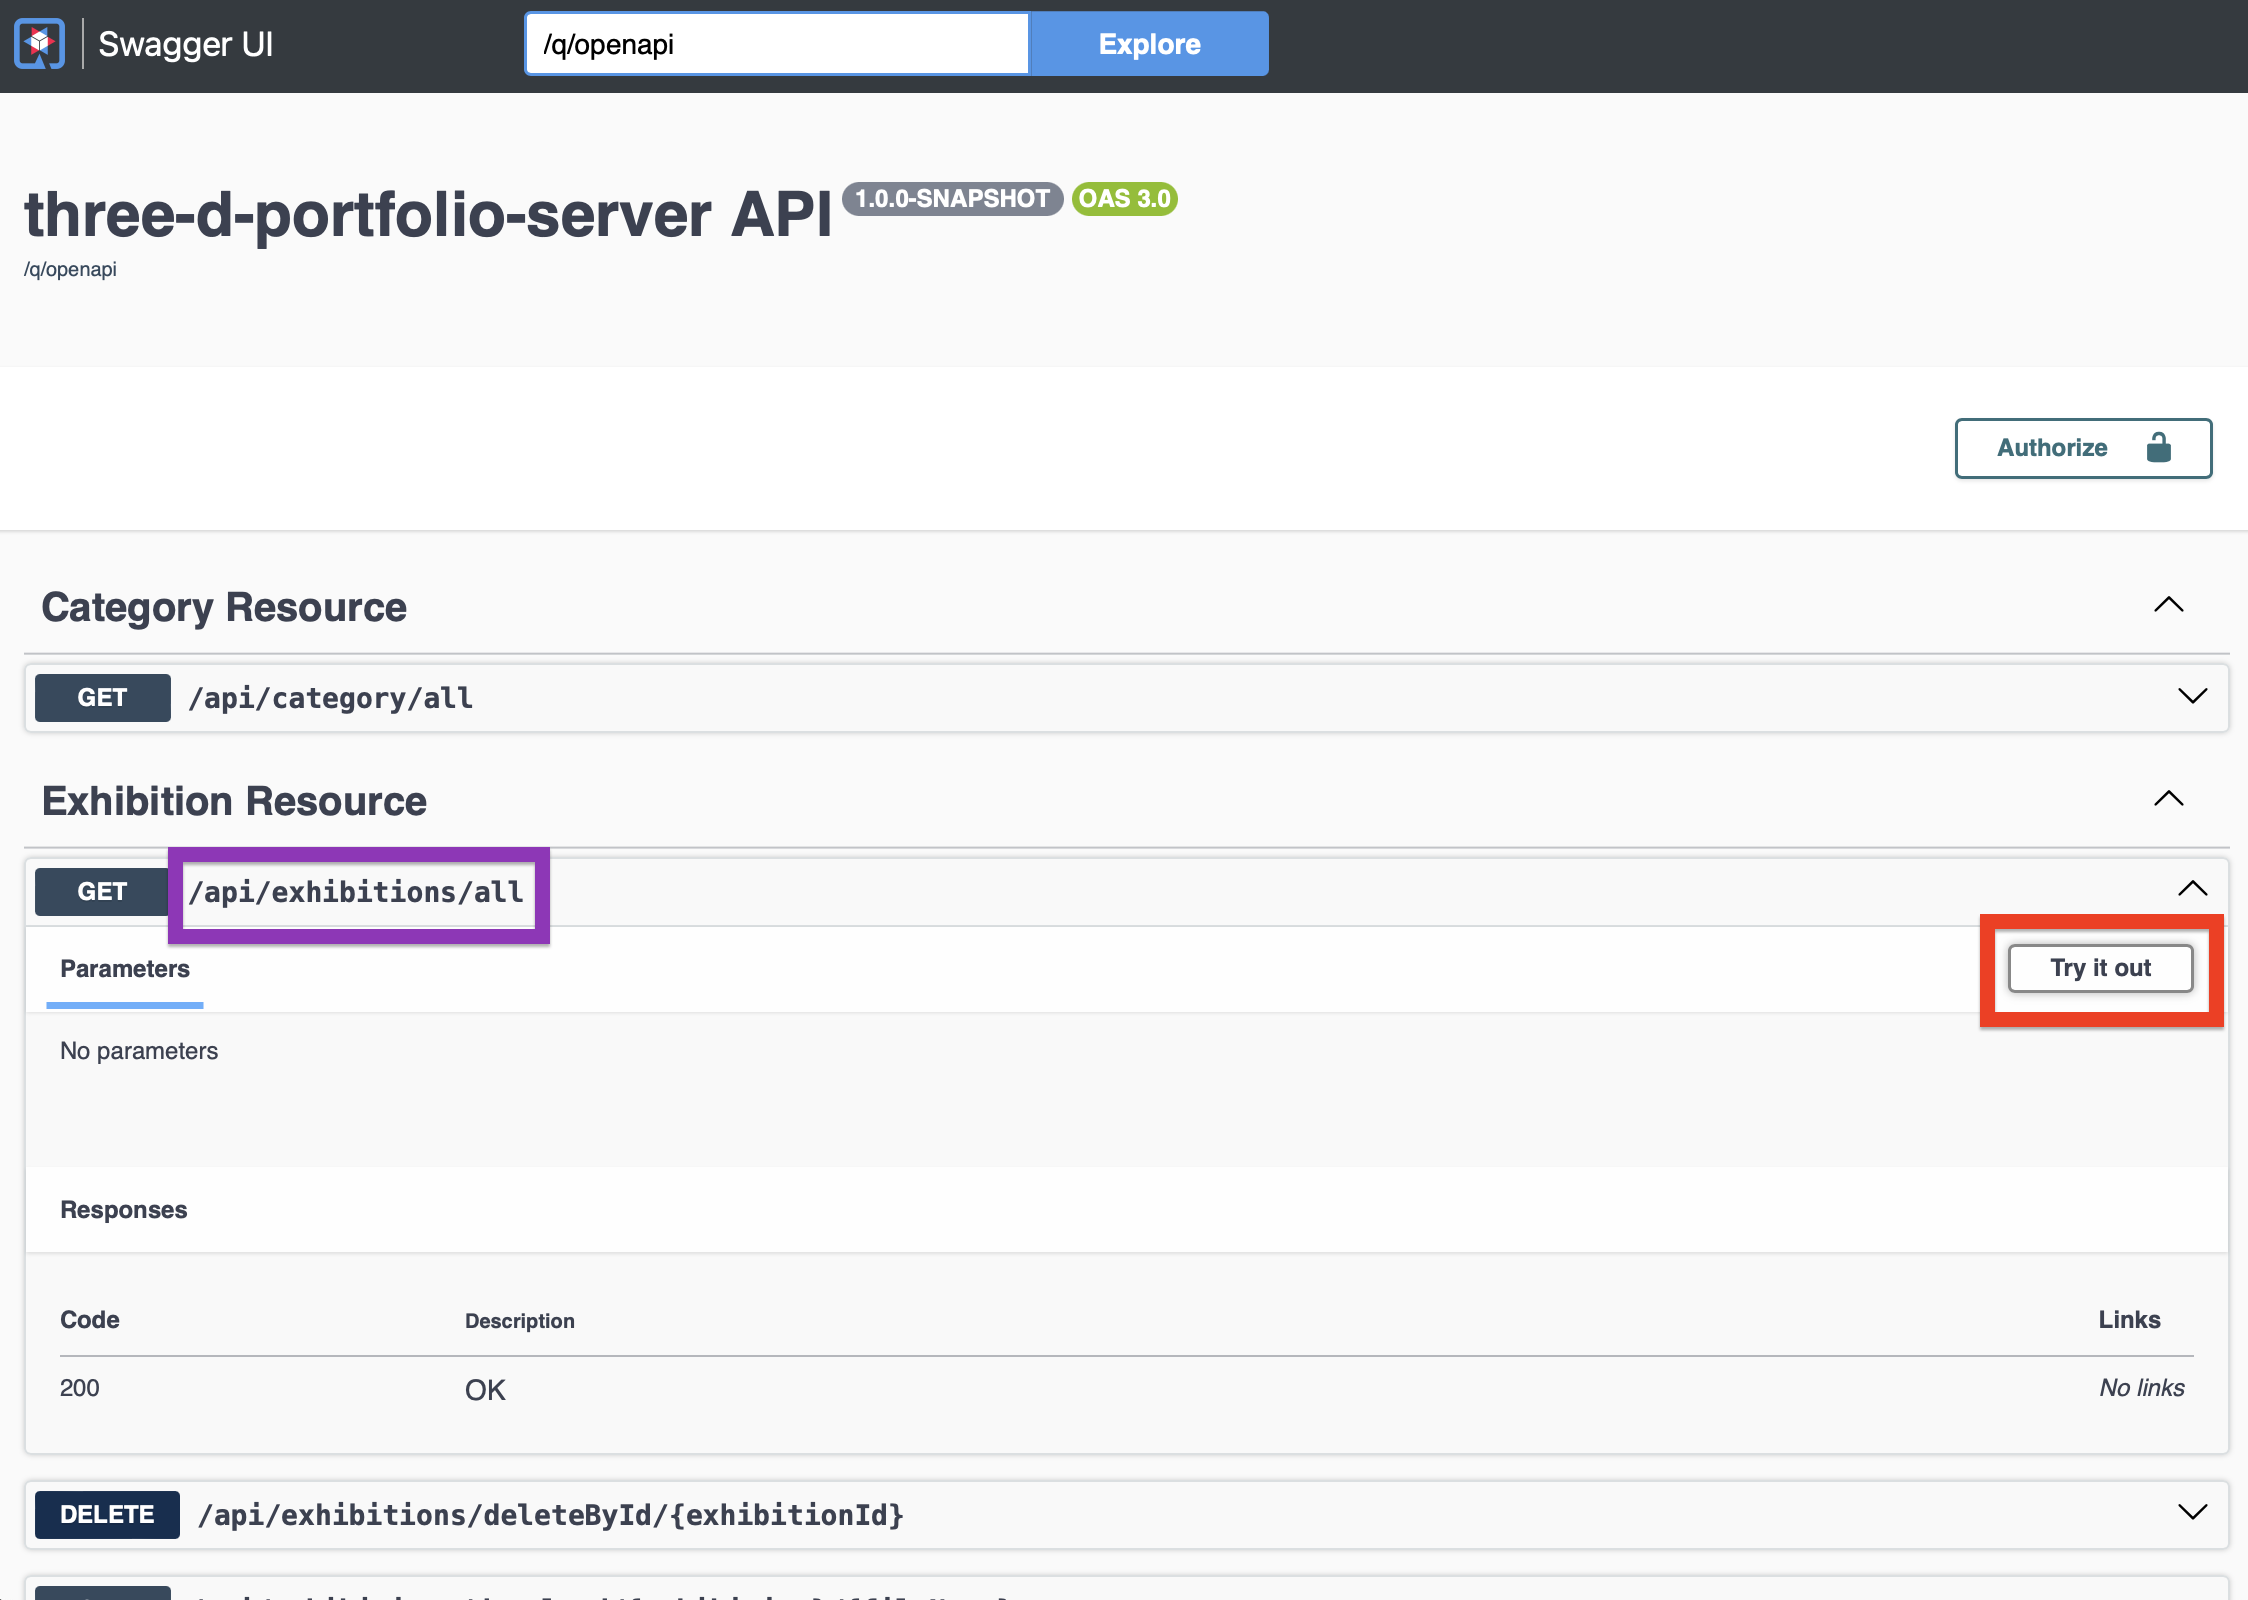
\includegraphics[scale=0.3]{pics/swaggerui.png}
    \caption{Übersicht der erstellten Schnittstellen}
    \label{fig:implementation:swaggerui}
\end{figure}

In Abbildung \ref{fig:implementation:swaggeruipost} lässt sich erkenen, dass die generierte Abfrage für numerische Werte standardmäßig \emph{0} und alphabetische Sequenzen \emph{string} einsetzt. 
Zweiteres ist kein Problem, da jedoch beim Anlegen jedes neuen Objekts die Id generiert wird, ist es einfacher, die Id aus dem Request zu entfernen. 
Falls jedoch ein bestimmter Wert für dieses Attribut gewünscht ist, muss die Einzigartigkeit der angelegten Entitäten beachtet werden. 
Ansonsten werden neue Objekt womöglich nicht gespeichert.

\begin{figure}
    \centering
    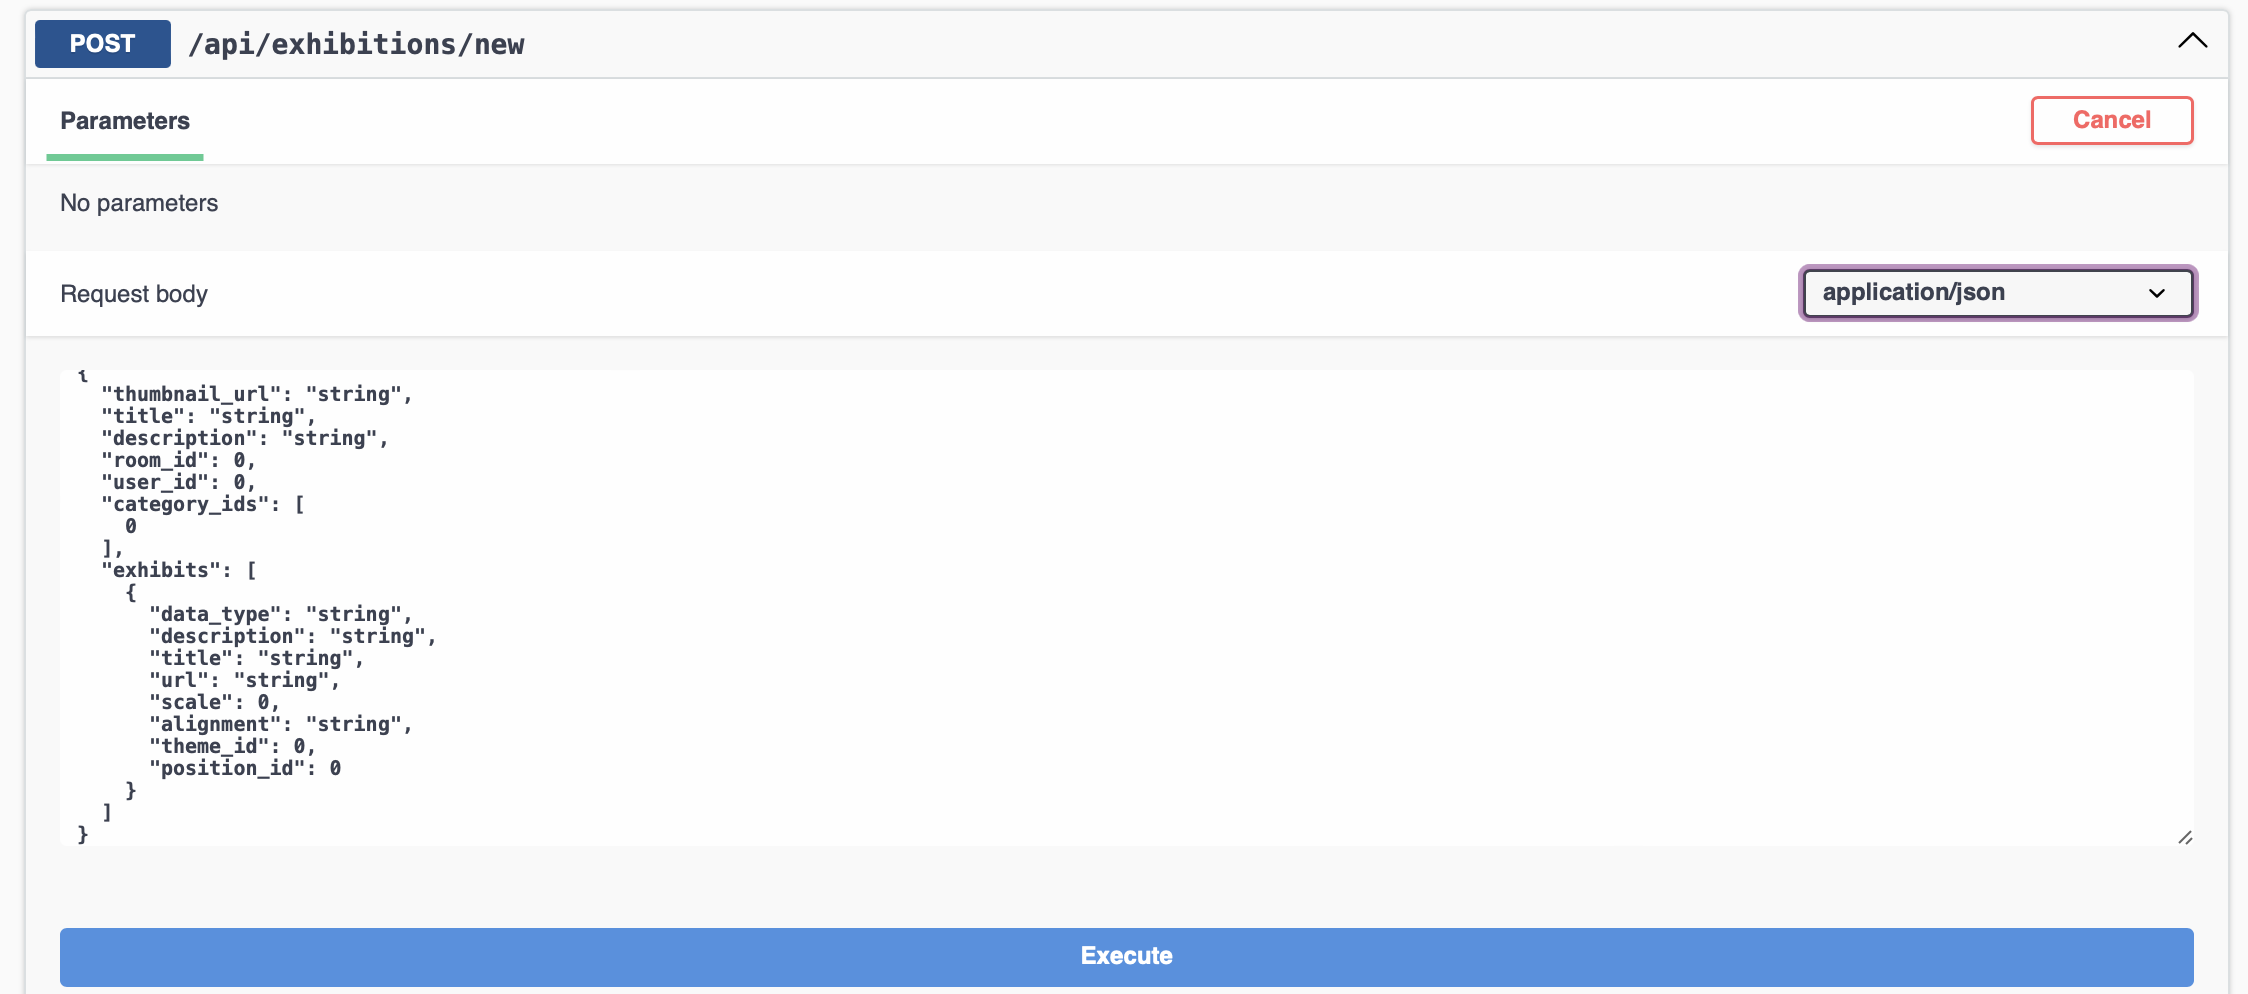
\includegraphics[scale=0.3]{pics/swaggeruipost.png}
    \caption{Automatisch generierte JSON-Anfrage}
    \label{fig:implementation:swaggeruipost}
\end{figure}

\subsection{Nach der Entwicklung}
Tests sind eine gute Möglichkeit, zu gewährleisten, dass die Applikation fehlerfrei ihre Aufgaben erledigt. 
Diese müssen eine breite Auswahl von möglichen Situationen abdecken.

In dieser Arbeit wird JUnit5 mit Mockito gearbeitet.
Mockito ermöglicht es, die Repositories zu rekonstruieren und dadurch alle Methoden aus diesen zur Verfügung zu stellen.

Durch die Priorisierung des Testvorganges während der Entwicklung, wurden die zusätzlich angelegten Testklassen nur für die wichtigsten Endpoints genutzt.

